\chapter{System Architecture and Detailed Design}

\section*{Introduction}
This chapter maps Qatra's requirements to deployable components and domain boundaries. It distinguishes logical responsibilities from physical deployment and explains the flows that require particular attention: authentication, appointment concurrency, event publication, authorization, and persistence.

\section{Global Architecture}
The user interacts with an external Angular single-page application. The repository contains exactly two deployable Spring Boot services: the donation service and the notification service. Identity, donor, center, appointment, emergency, matching, analytics, and audit responsibilities are modules inside the donation service rather than independently deployed microservices. Local Docker Compose uses Nginx as its gateway; the k3s environment uses Traefik \texttt{IngressRoute} resources. Domain events pass through Kafka to the notification service, while PostgreSQL and Redis provide persistence and fast operational state.

Figure~\ref{fig:logical-architecture} presents the responsibilities and the emphasized emergency path in a single icon-based view.

\begin{figure}[H]
\centering
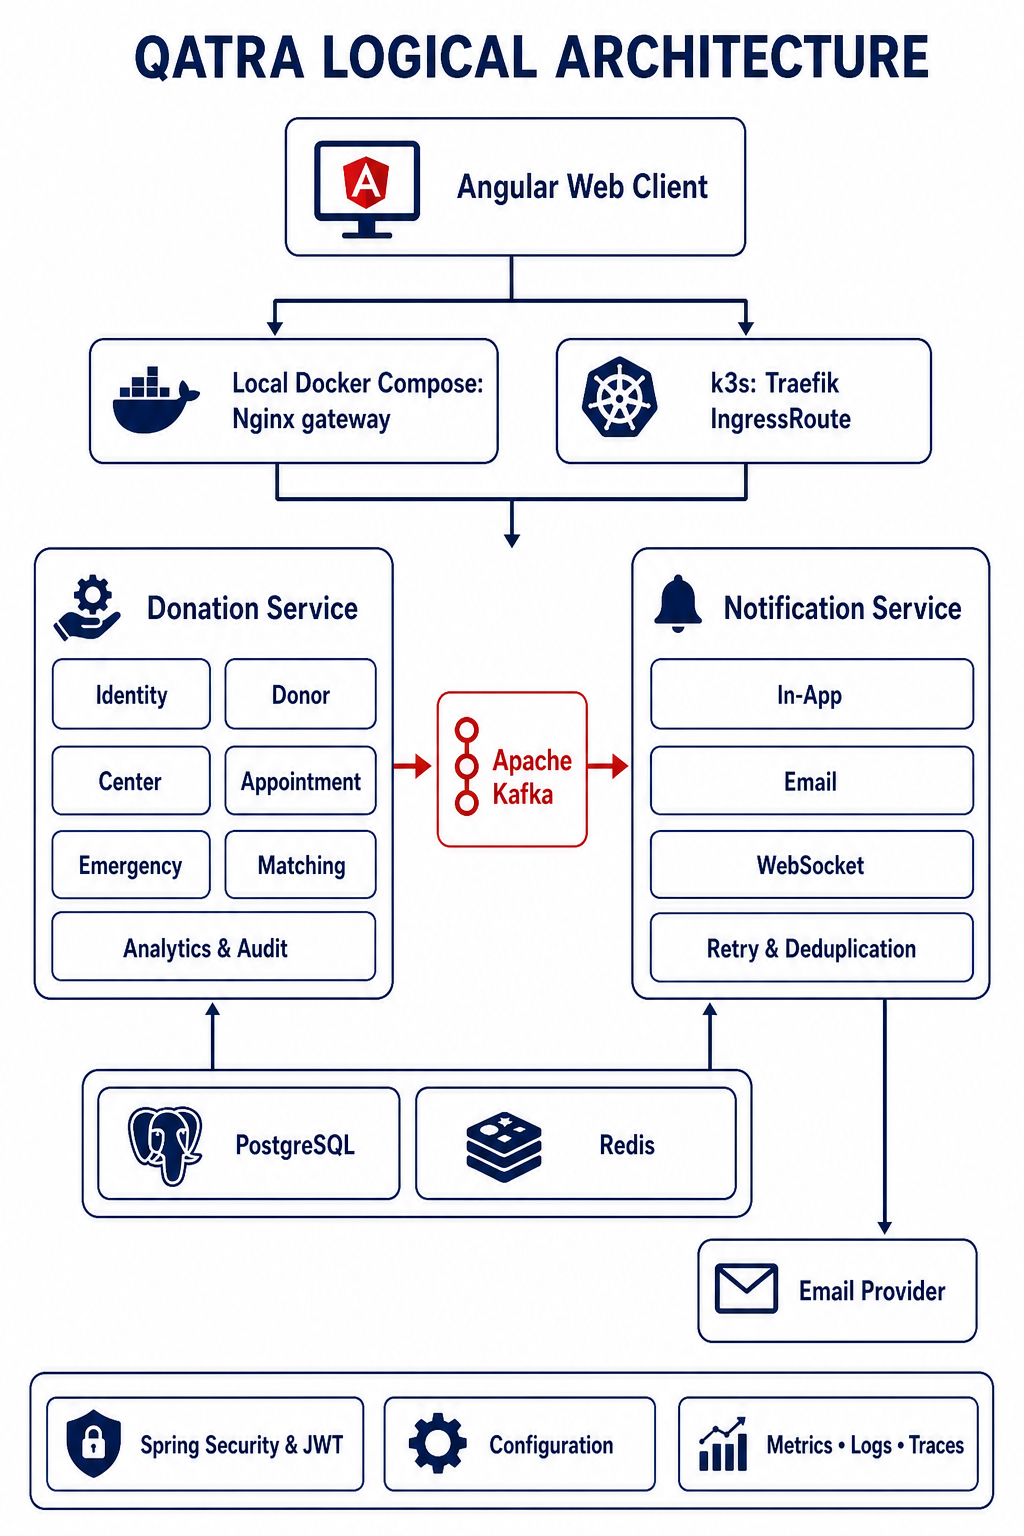
\includegraphics[width=0.82\textwidth,height=0.75\textheight,keepaspectratio]{assets/generated/logical-architecture-verified-portrait.png}
\caption{Verified logical architecture and deployable service boundaries of Qatra}
\label{fig:logical-architecture}
\end{figure}

The architecture avoids direct frontend access to databases or brokers. API boundaries centralize validation, authentication, DTO mapping, and error handling. The notification service is not a second source of truth for donation records; it reacts to identifiers and payloads required for delivery.

\section{Bounded Contexts and Modules}
The donation service contains domain-focused packages rather than a single generic service layer. The principal contexts identified from the repository are shown in Table~\ref{tab:contexts}.

\begin{longtable}{|P{3.0cm}|P{5.4cm}|P{5.0cm}|}
\hline
\rowcolor{tableheader}\textbf{Context} & \textbf{Responsibilities} & \textbf{Representative concepts}\\ \hline
\endfirsthead
\hline\rowcolor{tableheader}\textbf{Context} & \textbf{Responsibilities} & \textbf{Representative concepts}\\ \hline
\endhead
Identity/User & Registration, credentials, verification, roles, sessions & User, role, token, status\\ \hline
Donor & Profile, health, location, availability, eligibility, history & Donor profile, questionnaire, certificate\\ \hline
Center & Center lifecycle, staff, operating hours, slots & Donation center, staff profile, slot, closure\\ \hline
Appointment & Booking, rescheduling, screening, completion & Appointment, screening, outcome\\ \hline
Emergency & Urgent blood request, candidate response, progress & Emergency, blood type, deadline, status\\ \hline
Analytics/Audit & Metrics and state-change traceability & Audit log, center metrics\\ \hline
Notification & Delivery preferences, messages, real-time updates & Notification, channel, delivery state\\ \hline
\caption{Principal bounded contexts and responsibilities}
\label{tab:contexts}
\end{longtable}

Each context follows a recognizable direction of dependency: web adapters call inbound use cases; application services coordinate domain behavior; repository ports abstract persistence; JPA adapters map domain objects to entities. Proxies provide controlled access when one context needs information owned by another.

\section{Global Domain Model}
The global class model in Figure~\ref{fig:global-domain-model} consolidates the most important concepts from the implemented packages. It is intentionally a domain overview rather than a dump of every JPA field.

\diagram[0.58\textheight]{global-domain-model}{Global Qatra domain class diagram}

Important invariants include the following:

\begin{itemize}
  \item a slot belongs to one center and has finite capacity or state;
  \item an appointment associates a donor, a center, and a scheduled slot;
  \item screening precedes a completed donation outcome;
  \item eligibility depends on health restrictions and the most recent relevant donation state;
  \item an emergency declares a required blood type, location, deadline, and lifecycle status;
  \item candidate responses and delivery records must be attributable to the relevant emergency;
  \item audit records capture actor, action, target, and time for state-changing operations.
\end{itemize}

\section{Persistence Design}
PostgreSQL stores the relational domain. JPA entities and repositories provide persistence adapters, while mapper classes translate to and from domain models. This separation allows the domain vocabulary to remain stable if storage details change.

Indexes should follow actual query patterns: email and account state for authentication; center and date for schedules; donor and status for appointments; emergency status and deadline for active searches; blood type, availability, eligibility date, and location-related fields for matching; and timestamp, actor, and action for audit queries. Migration scripts and production index evidence should be treated as deployment artifacts; the report does not claim indexes that are not represented in the available schema.

\section{API and DTO Boundaries}
Controllers expose JSON-oriented contracts and delegate to application services. Request DTOs validate input such as appointment creation, screening, center updates, and status changes. Response DTOs prevent persistence entities from becoming public contracts. This boundary is particularly important for health and authorization data: the API should expose only the fields required by the caller's role.

Errors are represented through domain-specific error codes and centralized handling. This makes client behavior predictable and prevents internal stack traces from becoming an API. Pagination is used for lists that can grow, such as centers, appointments, users, emergencies, notifications, and audit records.

\section{Authentication and Authorization}
Authentication verifies credentials and issues signed tokens. Subsequent requests carry a token that is validated before the security context is established. Method or route authorization then checks the role and, where required, resource ownership or center membership.

\diagram[0.39\textheight]{authentication-sequence}{Authentication and protected request sequence}

Role checks alone are insufficient. A center administrator must not manage another center merely because the role matches. The application layer therefore needs contextual checks using the authenticated user and target entity. Account status, token expiry, and role changes must also be considered when accepting a token.

\diagram[0.34\textheight]{security-flow}{JWT security and role-based authorization flow}

\section{Appointment Consistency}
Appointment booking combines availability shown in the UI with authoritative server-side validation. Between display and confirmation, another donor may reserve the same capacity. The backend must therefore verify slot state within a transactional boundary and reject conflicts deterministically.

\diagram[0.40\textheight]{appointment-sequence}{Appointment booking, check-in, screening, and completion sequence}

The same workflow is represented as an activity diagram in Figure~\ref{fig:appointment-activity}, which emphasizes decisions and responsibility changes rather than message timing.

\diagram[0.58\textheight]{appointment-activity}{Appointment booking and donation activity diagram}

Rescheduling should behave as one business transition: validate the new slot, update or replace the reservation, and leave the previous slot in a consistent state. Check-in and completion are restricted to authorized staff. Completion triggers donation outcome and eligibility consequences rather than only changing a label in the UI.

\section{Physical Deployment Architecture}
The infrastructure repository declares one principal Kubernetes namespace, \texttt{qatra}. Inside it, the deployable business workloads are the donation service and notification service; PostgreSQL, Kafka, Redis, observability components, and administrative tools support them. Traefik \texttt{IngressRoute} resources expose the donation API, notification API, and notification WebSocket endpoint. The supplied manifests do not deploy the Angular frontend inside k3s, and they do not define Nginx as the Kubernetes ingress. Persistent storage is used where state must survive pod replacement.

\clearpage
\begin{figure}[H]
\centering
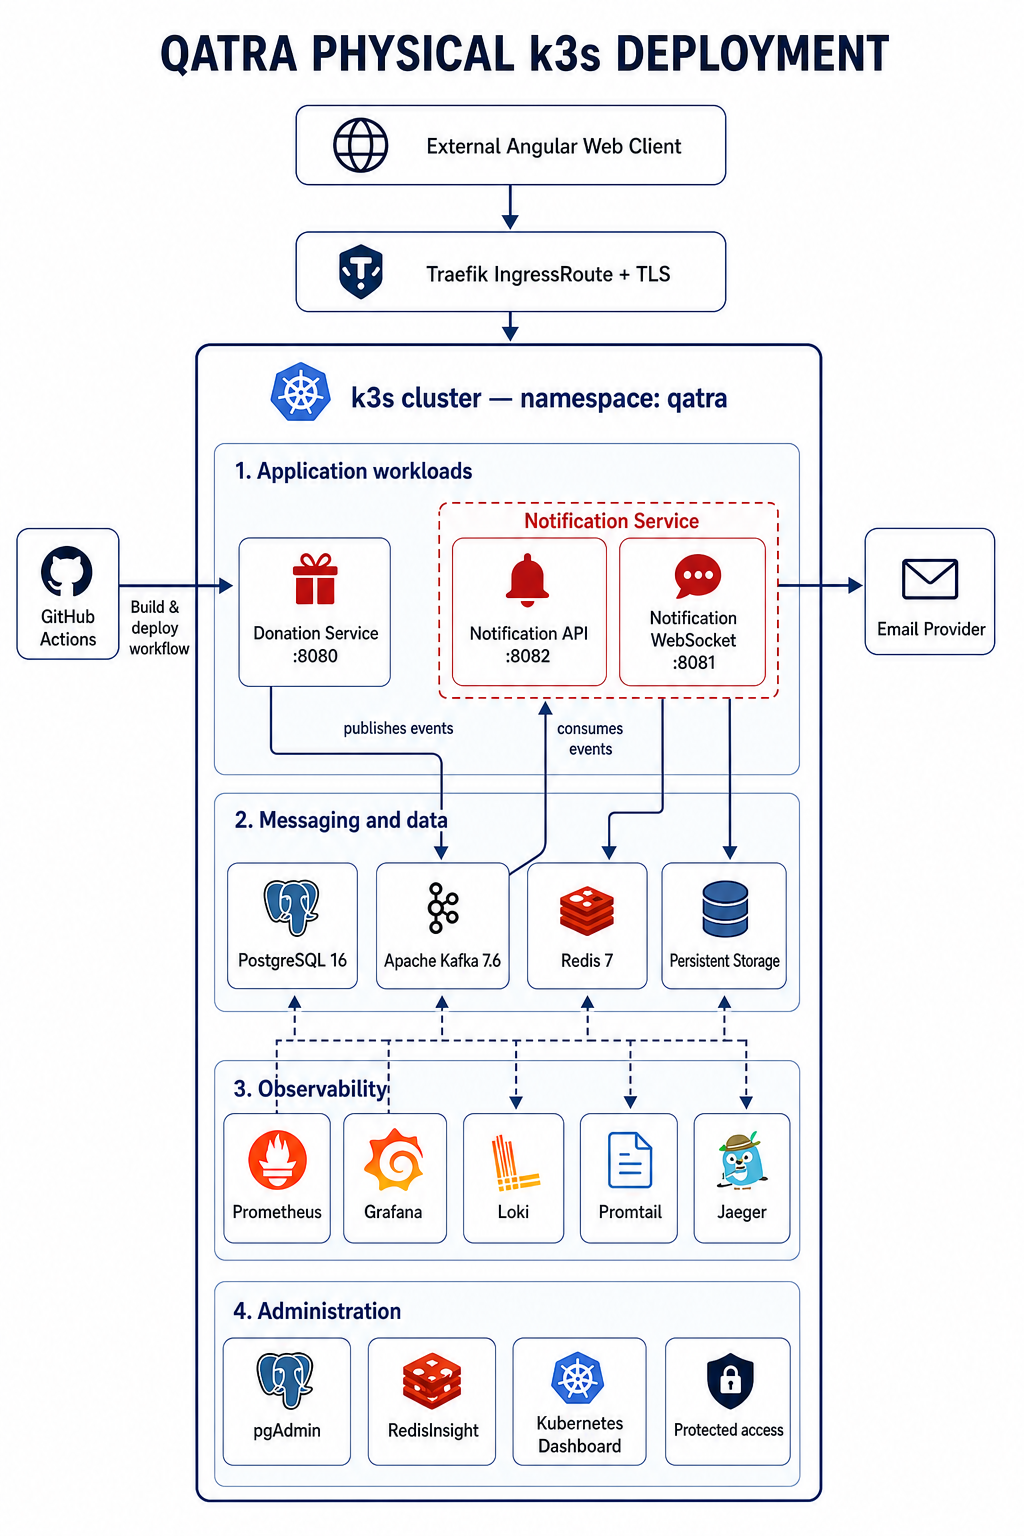
\includegraphics[width=0.82\textwidth,height=0.68\textheight,keepaspectratio]{assets/generated/physical-k3s-verified-portrait.png}
\caption{Verified physical k3s deployment in the single \texttt{qatra} namespace}
\label{fig:physical-deployment}
\end{figure}

Traefik provides the k3s entry point, whereas Nginx is limited to the local Compose gateway. Secrets should supply passwords, tokens, and API keys rather than embedding them in images or committed manifests. Readiness and liveness checks should distinguish a process that is running from a service that can accept work.

\section{Cross-Cutting Concerns}
Validation, error mapping, logging, correlation identifiers, audit events, metrics, and tracing apply across contexts. Correlation is particularly important when an emergency command produces a Kafka event and a later notification delivery. Without a shared identifier, logs remain technically centralized but operationally difficult to interpret.

\section*{Conclusion}
Qatra's architecture combines domain-oriented modules with a deliberately small service boundary, asynchronous notification flow, and production-like infrastructure. The following chapter uses the Kanban increments to connect this design to concrete user-facing capabilities.
